\chapter{Design}
\label{cha:design}

This chapter describes the design decisions taken in this project and how these work towards achieving the aims described in chapter \ref{cha:intro}.

\section{Overview}
As a methodology used during the project, the Agile Unified Process has been followed. This decision was taken because the process is iterative and it allows the developer to be flexible if circumstances change. Agile UP also focuses on producing working code over comprehensive documentation.

For splitting the tasks, we have been using \url{http://trello.com}, a free project management tool which allows creation of virtual boards and cards for each task, making it a virtual Kanban system.

For producing the UML diagrams, we have used \url{http://www.gliffy.com/}, an online tool which allows the user to create 5 diagrams for free.

\subsection{Project workflow}
The project has consisted of 4 phases:
\begin{itemize}
	\item \textbf{Phase 1} consisted of initial project documentation, background reading and an attempt to build a 3D car model to be used during the game. The sides of the car model were realistic enough, but I could not figure out how to build the front and the back, so I have used 3 free 3D models that I have found online. See Appendix \ref{appendix:3dobjects} for the sources of these objects.
	\item During \textbf{phase 2}, I have learnt more about Unity by following the \cite{walkerboys} tutorial. After that, \cite{flattutorials} was a good starting point to how one can create a car game in Unity. Some more advanced car physics ideas were inspired from \cite{carphysics}.
	\item \textbf{Phase 3} has seen the start of implementing the functionality from the developer's API of the Emotiv EPOC. The most important part was getting the training working inside the game. See figure \ref{fig:useCaseDiagram} for the use case diagram.
	\item In \textbf{Phase 4} the main concern was improving the user experience, getting some user testing done and allowing the player to choose between a variety of car models and colours.
\end{itemize}

\begin{figure}
  \centering
  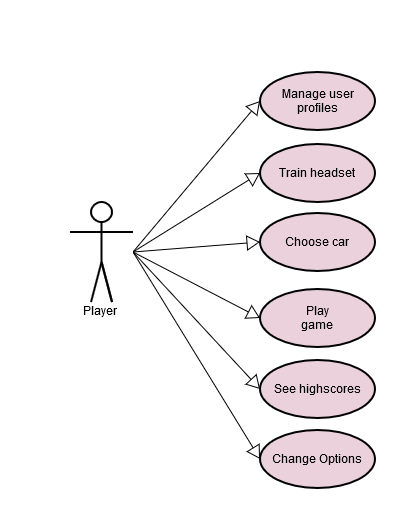
\includegraphics[height=350px]{usecasediagram.png}
  \caption{Use case diagram for CogniDriver.}
    \label{fig:useCaseDiagram}           
\end{figure}

\subsection{Requirements}

\subsubsection{Functional requirements}
In the final game, the player should be able to: 
\begin{itemize}
	\item Create/Delete/Change a player profile;
	\item Train the headset for neutral, push, pull, left, right states;
	\item Allow the user to accept/reject/reset a training session;
	\item Display the updated skill level after each training session;
	\item Provide visual feedback as to how well the training is going by using an animated object;
	\item Alert the user in the training scene if a training profile is not complete;
	\item Display the top 10 highest scores for Keyboard mode play and Cognitiv mode play;
	\item In the Options tab, allow the user to change sound volume, sound effects volume and whether the game will be played in fullscreen;
	\item Allow the user to change between Keyboard, Cognitiv and Gyro play modes;
	\item Provide instructions on how to train and play the game;
	\item Pause/Exit the game;
	\item Allow the selection of a car model and colour;
	\item Race yourself during the game play.
\end{itemize}

\subsubsection{Non-functional requirements}
\begin{itemize}
	\item The game should be portable (i.e. playable on multiple operating systems);
	\item Once loaded, there should be no long waiting periods of time.
\end{itemize}

\subsection{Separation of concerns}
The Model-view-controller architecture has been used with the purpose of separating the concerns such that the controller (the script) is manipulating the model (car or environment) which then updates the view (the user interface).

\section{Design Patterns}

\textbf{Abstract Factory} has been used to create cars from the abstract \texttt{Car} class. \texttt{AudiR8} and \texttt{FerrariCalifornia} are thus inheriting from \texttt{Car}. See figure \ref{fig:classDiagram} for the UML class diagram.

\textbf{Strategy} is used to decide which car control options to follow depending on the game play mode: Keyboard, Cognitiv or Gyro. It is also used in the car model choice.

%\begin{landscape}
\pagestyle{plain}
\begin{sidewaysfigure}
  \centering
  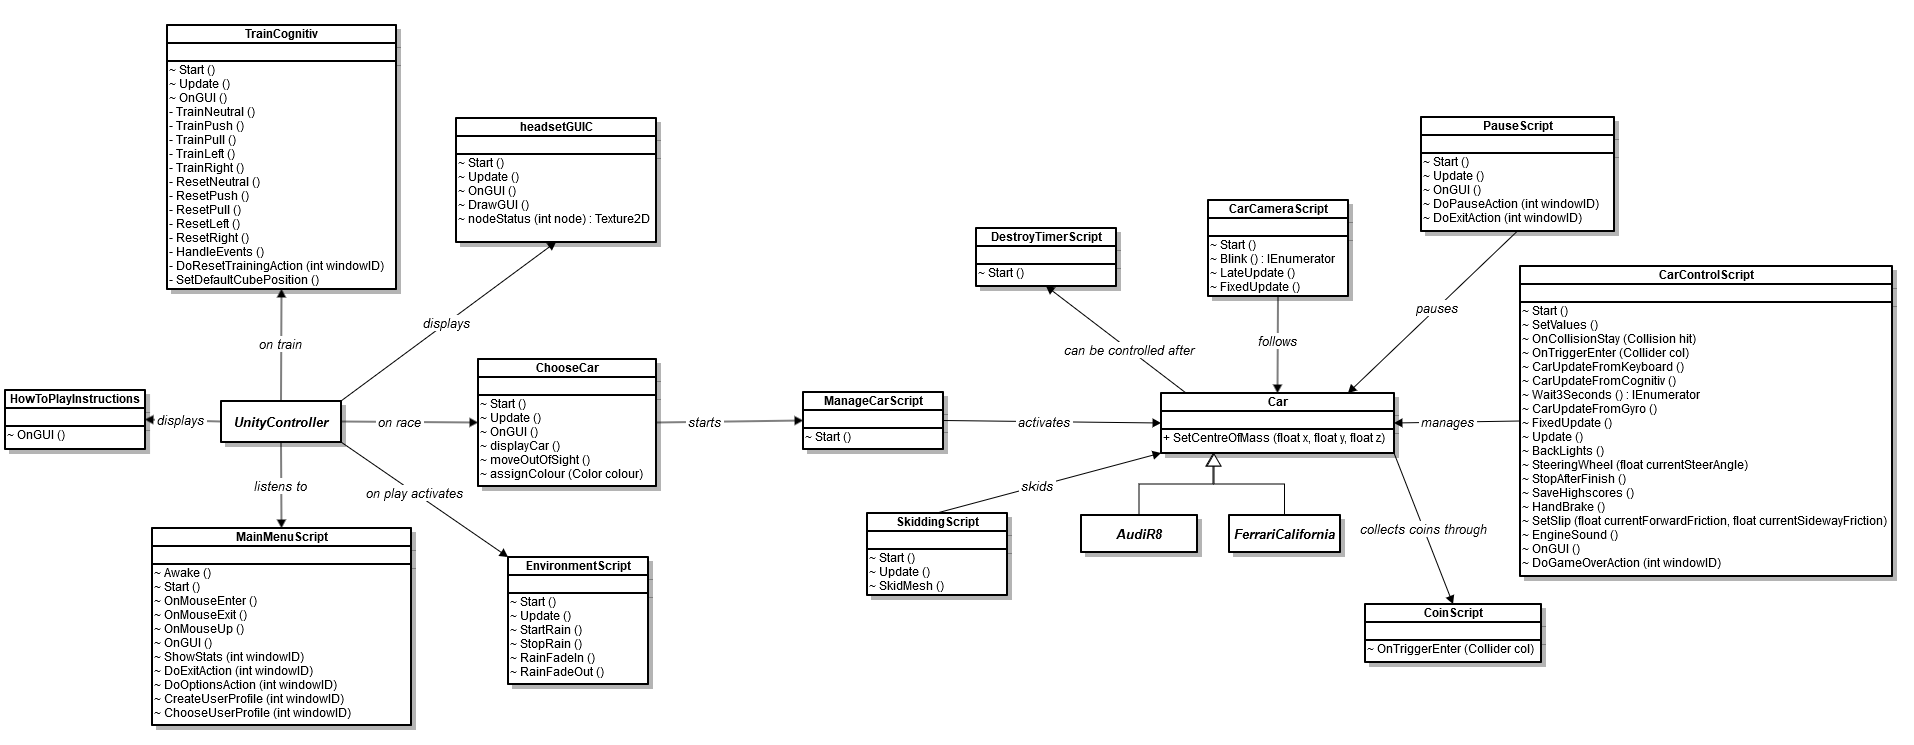
\includegraphics[width=750px]{CogniDriverDomainClassDiagram.png}
  \caption{Domain class diagram for CogniDriver. The instance variables have been omitted for simplification.}
    \label{fig:classDiagram}           
\end{sidewaysfigure}
%\end{landscape}